\section{Results}

\begin{figure}[H]
    \centering
    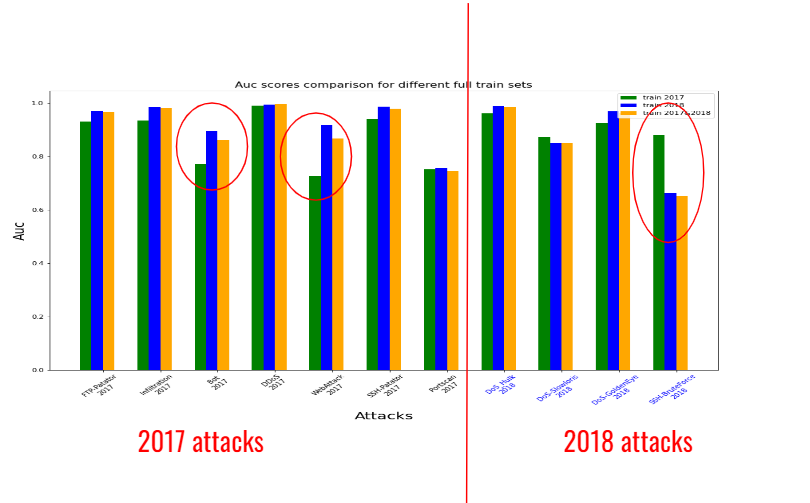
\includegraphics[width=1\linewidth]{augment.png}
    \caption{}
\end{figure}

In our experiments, we see that using foreign datasets during training increases the AUC score. In Figure 1, when using the 2017 dataset as the test set, training with 2018 dataset or training with both 2017 and 2018 datasets outperforms training with just 2017 dataset in most attacks scenarios. Similarly, when using the 2018 dataset as the test, training with 2017 datasets or combining both datasets outperforms training with just 2018 dataset. We have highlighted the attacks in which augmenting data with foreign datasets will increase performance. As such, we conclude that in many case, augmenting data will benefit the detection system.

\begin{figure}[H]
    \centering
    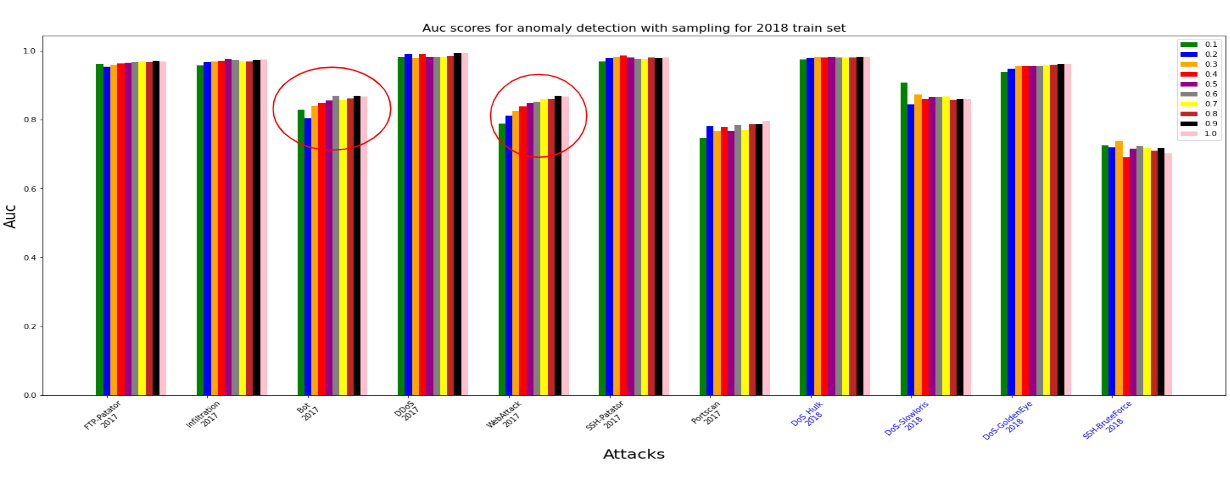
\includegraphics[width=1\linewidth]{amount.png}
    \caption{}
\end{figure}

In Figure 2, we see that only in certain attack scenarios does the amount of the data impact our result. Specifically, the BotNet 2017 and WebAttack 2017 showed strong evidence that increasing the training set size will better the AUC score. In other scenarios, we don't see a strong trend and the effect of dataset size on the AUC score is inconclusive.

\begin{figure}[H]
    \centering
    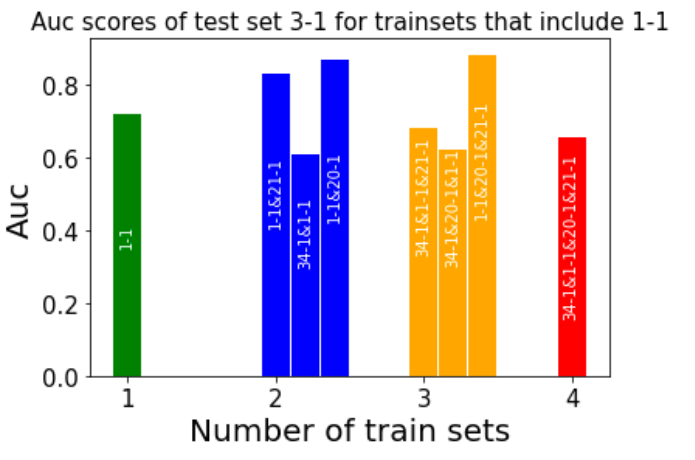
\includegraphics[width=1\linewidth]{data.png}
    \caption{}
\end{figure}

In Figure 3, we augment the data with different foreign datasets and we see that there is huge variance in the resulting AUC scores, meaning that the type of data that is shared with the trainer matters too. It's inconclusive exactly what type of data will benefit the most in different attack scenarios.

\label{sec:results}
